\documentclass[9pt,preprint]{sigplanconf}
% \documentclass[pldi,10pt,preprint]{sigplanconf-pldi16}

% The following \documentclass options may be useful:

% preprint      Remove this option only once the paper is in final form.
% 10pt          To set in 10-point type instead of 9-point.
% 11pt          To set in 11-point type instead of 9-point.
% authoryear    To obtain author/year citation style instead of numeric.

\usepackage{graphicx}
\usepackage{caption}
\usepackage{subcaption}

\begin{document}

\newcommand{\charcoal}{Charcoal}
% \newcommand{\charcoal}{BlindReview}
\newcommand{\noyield}{\texttt{no\_yield}}

\special{papersize=8.5in,11in}
\setlength{\pdfpageheight}{\paperheight}
\setlength{\pdfpagewidth}{\paperwidth}

\conferenceinfo{CONF 'yy}{Month d--d, 20yy, City, ST, Country}
\copyrightyear{2014}
\copyrightdata{978-1-nnnn-nnnn-n/yy/mm}
% \doi{nnnnnnn.nnnnnnn}

\titlebanner{Preprint.  Please do not redistribute}        % These are ignored unless
\preprintfooter{Preprint.  Please do not redistribute}   % 'preprint' option specified.

\title{Atomic or Interruptible?
Let the Caller Decide!}
\subtitle{or, the Abstraction Problem in Cooperative Concurrency}

%% \authorinfo{Blind Review}
%%            {Blind Review University}
%%            {BlindReview@BlindReview.edu}
\authorinfo{Benjamin Ylvisaker}
           {Colorado College}
           {ben.ylvisaker@coloradocollege.edu}

\maketitle

\begin{abstract}

The sophistication of multitasking patterns in mainstream software has increased in recent years, thanks to the increasing richness of network communication, physical world interaction and multi-process software architectures.
These trends have pushed language designers to reevaluate the trade-offs in multitasking abstractions.
For example, though coroutines have been known for decades, many widely used programming languages have only recently added native support for them.

This paper introduces a new multitasking abstraction called pseudo-preemptive threads that combines the software engineering benefits of several existing options.
This paper has a detailed comparison of pseudo-preemptive threads with established multitasking abstractions.
It also describes novel implementation techniques: a new call frame allocation strategy and a fast task yield implementation.
Finally we report performance results for several microbenchmarks using the prototype implementation of pseudo-preemptive threads that we developed.

\end{abstract}

% \category{CR-number}{subcategory}{third-level}

% general terms are not compulsory anymore,
% you may leave them out
% \terms
% term1, term2

% \keywords
% keyword1, keyword2

%% Why Events, Preemptive Threads and Coroutines are All Bad Ideas\footnotemark
%% \footnotetext{This tongue-in-cheek subtitle is a reference to Ousterhout \cite{Ousterhout1996} and von Behren, et al. \cite{Behren2003a}}

\section{Introduction}

Multitasking (or asynchrony) has been a facet of application software forever.
Common use cases include reacting to user input (keyboard, mouse, touch, etc.), communicating with other machines over a network, managing ``slow'' physical-world devices, and interacting with external processes.
In recent years the richness of multitasking in mainstream applications has increased along with a few trends: increasing use of network services (e.g. Web APIs), increasingly rich physical world interaction (especially with mobile devices), and the increasing use of microservices as a software architecture.
This has put renewed pressure on programming languages to provide good ways to write efficient and reliable multitasking software.
This paper introduces a new multitasking primitive that has software engineering advantages over existing alternatives.

The software industry has not come to consensus yet on best practices for implementing multitasking software.
One well-known option is threads.
Unfortunately, programming with threads is notoriously hard; it is easy to introduce subtle and non-deterministic bugs that can be very hard to diagnose and fix [cite].
Though threads are useful for some applications, in this paper we focus on application domains in which getting multithreaded programming right is too expensive.

As a safer alternative to threads, much of the software industry has opted for cooperative concurrency.
The most commonly used primitives are event dispatchers, coroutines, async procedures/methods, and cooperative threads.

In modern application development practice, it is common to reuse collections of modules/libraries, often with deep chains of dependencies among libraries.
In the context of a cooperative concurrency framework, there is an extremely important question a programmer should ask when invoking an abstraction provided by a library:
Is it possible for control to switch to a different task during the execution of this abstraction?
In other words, is the abstraction atomic or interruptible?

In the context of libraries that build on other libraries, we need to take this question further:
Can I write an abstraction that can be invoked in an atomic/interruptible way by client code, \emph{and} invokes abstractions provided by libraries that I do not have control over?
In other words, can I build an atomic abstraction on top of an interruptible one, and/or vice versa?

We claim that existing cooperative concurrency primitives all have problems with regard to these atomic/interruptible abstraction questions.
We propose a new primitive called \emph{activities} that we show aleviates these abstraction problems.
In implementation terms, activities are cooperative threads plus implicitly inserted yields and an atomic block primitive.

We implemented activities in two contexts.
First, we implemented activities as a library in JavaScript.
This is possible because JavaScript already has a coroutine-like primitive (as of ECMAScript 6) and a global event dispatcher.
This implementation's syntax is not ideal, because it is not ``native'' to the language.
However, it is possible to integrate this implementation fairly cleanly with existing JavaScript code, which makes it easier to investigate software engineering questions.

The second implementation is a dialect of C.
We built this implementation to investigate the performance overhead of activities in terms of both memory and time.
We introduce a new call frame allocation strategy called \emph{hot stacking}, which provides low memory and time overhead.
This allocation strategy is enabled by activities in the sense that we believe implementing it in the context of other thread-like primitives would be substantially more complex and potentially have bad uncommon case performance characteristics.

%% It is hard to write complex multitasking software that is reliable, composable, and efficient.
%% It is even harder to maintain such software.
%% The programming world has not yet come to consensus on the best abstraction for multitasking, because there are strong competing constraints and no obvious way to satisfy them all simultaneously.

%% This paper focuses on the interraction between cooperative concurrency mechanisms and procedural abstractions (i.e. functions, methods, subroutines, etc.).
%% Procedural abstraction is foundational in software engineering.
%% When we consider procedures in the context of multitasking software, a very important question presents itself: When a caller invokes a procedure, will that invocation be atomic or interruptible?

%% Clearly not all invocations can be atomic.
%% If that was the case, then the running task would never allow control to transfer to another task, and the softare would not be multitasking.
%% In many cases programmers prefer that invocations be atomic.
%% If they are interruptible, then reasoning is much harder.

%% The time is ripe to reevaluate the tradeoffs in multitasking abstractions, because of two trends.
%% Mainstream application software is getting more complex in terms of multitasking.
%% This is because network communications, physical world interactions and multi-process software architectures (e.g. microservices) have all become more common in recent years.

%% The other trend is relevant to the embedded systems world.
%% Embedded software has long had a stronger focus on multitasking than mainstream applications.
%% However, embedded software is becoming more and more complex; people are expecting much more general-purpose computing functionality from their ``smart devices''.
%% Historically, highly constrained multitasking abstractions, like main loop scheduling, were popular in embedded software.
%% But these abstractions get harder to work with, the more complex the software is.

%% As result of these two trends there is a greater need than ever for multitasking abstractions that make it as easy as possible to make complex software.

%% Writing efficient, reliable and maintainable multitasking software is important and hard.
%% Many abstractions have been popular over the years for multitasking, but none has ever been universally accepted XXX.
%% Two trends are again pushing on the software engineering challenges of multitasking and motivating programmers to seek alternatives.

%% In mainstream application software, network communication, physical world interaction and decompostion into communicating processes (microservices) are all becoming more common.
%% These features have long been prominent in embedded software, but in that community the most common patterns for multitasking were very inflexible (e.g. main loop scheduling).
%% Embedded systems are rapidly becoming more complex (see new buzz phrases like Internet of things and cyber-physical systems).
%% These more complex systems make using inflexible multitasking abstractions more painful.

%% Modern mainstream software is substantially more concurrent than its forebears, in the sense that frequent network communications, rich physical world interactivity, and factoring applications into communicating processes (microservices) have become common.
%% Note that in this paper we are mostly not concerned with concurrency in the sense of running software on multiple processors simultaneously (i.e. parallelism).
%% We use \emph{multitasking} to refer to the subset of concurrency that is not parallelism.

\subsection{Activities}

This paper introduces a new multitasking abstraction called \emph{pseudo-preemptive threads} (or \emph{activities}) that has software engineering benefits compared to existing alternatives.
From a programmer's perspective, activities are most similar to user-level preemptive threads.
The primary difference is that user-level threads can be preempted at any time, but activities have a coarser granularity of scheduling that is defined in terms of the source language, not the implementation.
This paper also introduces a new call frame allocation strategy called hot stacking that has close to zero per-thread memory overhead, yet still performs well for the most frequent calls/returns.

The brief version of how activities are implemented is that they are cooperative threads, but the compiler/interpreter automatically inserts yields, to make them appear closer to preemptive.
There is a dynamically scoped \emph{no-yield} primitive that allows programmers to enforce atomicity for arbitrary blocks by overriding/suppressing yields.
From a programmer's perspective the no-yield primitive is similar to \emph{atomic} in transactional memory abstractions.

Differences between multitasking abstractions can be quite subtle, even if the software engineering implications of those differences are profound.
In the next section we briefly describe several established multitasking abstractions in preparation for a detailed discussion later of what distinguishes activities from its cousins.

To validate the ideas presented in this paper, we implemented activities in a dialect of C called \charcoal{}.
In particular, we focus on two efficiency issues: memory scalability and yield performance.
We describe the important parts of our implementation and present results from a collection of microbenchmarks to show that activities pay very little performance overhead for their software engineering benefits.
The \charcoal{} implementation and all the benchmarking code reported in this paper are available publicly on GitHub [\texttt{github.com/benjaminy/Charcoal}].

% We also tweaked two real-world multithreaded C programs to use activities instead of threads to explore the software engineering implications.

\subsection{Contributions}

This paper has three primary contributions:

\begin{itemize}
\item Introduction of \emph{pseudo-preemptive threads/activities}.
\item Introduction of \emph{hot stacking}.
\item A novel high-performance implementation of yield.
\end{itemize}

%% There are many existing multitasking abstractions, and some of the distinctions between them and activities are subtle.
%% So we start with a description and critique of existing multitasking abstractions


\section{Atomic or Interruptible?}

In this section we describe the importance of atomicity and interruptibility in the context of cooperative concurrency frameworks.
We also describe the problems that existing frameworks have with these concepts and abstraction.

\subsection{On Atoms and Interrupts}

Consider the following simple code snippet:

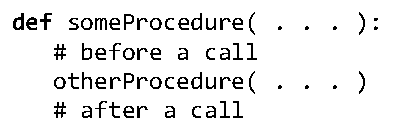
\includegraphics[scale=0.7]{trivial_call}

Reasoning (both human and automated) about the call to \texttt{otherProcedure} is much easier if that call is atomic.
In that case, the only way the program's global state can change is as a result of actions performed by \texttt{otherProcedure} (and procedures it calls).
If \texttt{otherProcedure} is interruptible, the program's global state can change as a result of actions taken by some concurrent task.

On the other hand, if the execution of \texttt{otherProcedure} might take a long time\footnotemark{}, then making the call atomic runs the risk of making the program unresponsive to events that happen while \texttt{otherProcedure} is running.
In this case, we probably want \texttt{otherProcedure} to be interruptible.

\footnotetext{It does not matter whether this is because \texttt{otherProcedure} is computationally intensive or because it waits for something from outside the program itself.}

The tension between atomicity and interruptibility is problematic for library procedures that should be atomic in some calling contexts and interruptible in others.
For example, consider a data structure \emph{map} procedure that applies a function to each item in an aggregate structure.
In a context where the caller knows that the data structure is small and the function to be applied is fast, the caller probably strongly prefers that the whole map operation be atomic; this simplifies reasoning with little risk of unresponsiveness.
On the other hand, in a context where the caller knows that the data structure is large or the function to be applied is slow, the caller probably strongly prefers that the whole map operation be interruptible.

Library authors are faced with a serious dilemma here.
One obvious and deeply flawed solution is for library authors to provide two versions of each operation that callers might reasonably want to be either atomic or interruptible.
Source code duplication.
This idea is especially painful in modern highly modular ecosystems, because the duplication would be everywhere.

Atomicity and interruptibility are important in different ways and in direct conflict with each other.
Atomicity is good because it allows programmers (and analysis tools) to reason about chunks of program behavior without the possiblity of interference from concurrent tasks.
Programmers are notoriously bad at reasoning about potential interference during the execution of some abstraction, so the more a framework can guarantee that cannot happen, the better.

On the other hand, all cooperative concurrency frameworks need interruption of some kind.
Unless all tasks can be guaranteed to run in a short amount of time (which is not possible in the context of a general purpose language), there will eventually be a need to choose between interrupting one task and being unresponsive to another task.

As a general guideline, we would like interruptions to happen as infrequently as is practical, without causing unresponsiveness.

\subsection{Coopertive Threads}

Cooperative threading frameworks provide a spawn primitive that creates a new task.
Only one cooperative thread can be running at a time and the active thread cannot be involuntarily interrupted by the system.
Cooperative threads must explicitly invoke a \emph{yield} primitive that can choose to transfer control to a global scheduler (and from there to any runnable thread).

The problem with cooperative threads is that any procedure might invoke yield, which would make it interruptible.
A procedure is also interruptible if any procedure it invokes is itself interruptible.

Not knowing whether a given library call is interruptable or not makes it hard to write reliable client code.
Even if libraries provide some (reliable) annotation about whether an abstraction is atomic or iterruptible, cooperative threading frameworks make it \emph{too easy} to change this in the process of maintanence and evolution of a library.
Changing an abstraction from atomic to interruptible (or vice versa) has the potential to break client code.

\subsection{Events}

In contrast to cooperative threads, event dispatching frameworks make it painfully clear what is atomic and what is interruptible.
All procedures/methods/functions are atomic; there is no mechanism, voluntary or otherwise, for interrupting a running procedure.

\section{Established Multitasking Abstractions}

In this section we give brief definitions of established multitasking abstractions.
Jargon is used somewhat inconsistently in this domain, so we establish how we use terms in this paper.
This section is intended to be free of judgments about the strengths and weaknesses of these options.
Its main purpose is to serve as a foundation for the arguments in the next section that pseudo-preemptive threads are a distinct, new multitasking abstraction.

The main dimension that we focus on is scheduling flexibility.
The more constrained scheduling is, the \emph{easier} it is to avoid defects like atomicity violations and incorrect ordering.
However, highly constrained scheduling also makes it \emph{harder} to avoid defects like starvation and unintended blocking of tasks.
Abstraction with more flexible scheduling have exactly the complementary strengths and weaknesses with regard to concurrency defects.
There is no way to completely guarantee the absence of these defects; the best we can do is minimize risk.

As a side note, software architectures that emphasize independence of tasks, like functional style programming and isolated processes tend to be more resistant to many kinds of concurrency bugs.
However, \emph{inter}dependence of tasks (e.g., frequent shared memory access and synchronization) is common in modern practice, and we do not expect that to change radically in the near future.

Experts can safely skip the remainder of this section.

\begin{table}
  \centering
  \begin{tabular}{|l|}
    \hline
    Main loop scheduling \\
    \hline
    Events \\
    \hline
    Coroutines (stackless) \\
    \hline
    Cooperative threads \\
    \hline
    Pseudo-preemptive threads/activities \\
    \hline
    User-level threads (preemptive) \\
    \hline
    System threads \\
    \hline
    System threads + transactions \\
    \hline
  \end{tabular}
  \caption{The multitasking abstractions that we compare pseudo-preemptive threads to in this paper.
  They are ordered by the task switching/scheduling flexibility of the abstraction, with the least flexible at the top.}
  \label{table:abstractions}
\end{table}

\textbf{Main loop scheduling}.
Main loop scheduling is used heavily in embedded systems.
In this architecture, an application's main procedure is an infinite loop that calls a statically-fixed sequence of procedures.
There is very little scheduling flexibility in main loop scheduling.

\textbf{Events}.
In event-based multitasking, a central \emph{dispatcher} or \emph{event loop} calls handler procedures (\emph{callbacks}) in response to events like I/O operations and timers expiring.
A defining characteristic of events is that at most one callback can be running at a time.
If an event happens while a callback is running, the next callback must wait until the current one returns.
Many kinds of atomicity violations are impossible with events, because there is no concept of interruption or even voluntary context switching during the execution of a callback.
Starvation is a serious concern, because a callback that runs for a long time or blocks will prevent other tasks from running.

\textbf{Coroutines}.
The increasingly sophisticated multitasking in mainstream software and the well-known problems with events and threads have forced language designers to explore alternatives in recent years.
The most widely used alternative is \emph{coroutines}\footnotemark{}.
Examples include async/await, which was added to C\#/.Net in 2012; function generators (\texttt{function*}), which were added to JavaScript with ECMAScript 6 (standard published in 2015); even the C++ community is considering adding support for coroutines (N4286, proposed for C++17).
Coroutine implementations are not \emph{new}; for example, Modula-2 had coroutines in the 1980s.
However, relatively few of the most widely used languages natively supported coroutines until recently.

\footnotetext{In many cases language designers chose terms other than \emph{coroutine} for reasons that we can only speculate about.}

In a coroutine framework, programmers \emph{manually} partition procedures (methods, functions, subroutines, whatever) into \emph{regular procedures} and coroutines.
``Calling'' a coroutine actually spawns a task that runs concurrently with the executing code.

Unlike event callbacks, multiple coroutines can be in progress simultaneously.
Context switching between coroutines is only permitted when a \emph{yield} primitive is \emph{explicitly} invoked.
Regular procedures \emph{cannot} yield; in other words, regular procedure calls are atomic.
A somewhat non-obvious consequence of this atomicity is that coroutines spawned by regular procedures cannot start running until the procedure returns back to a coroutine (possibly through some stack of procedure calls).

\textbf{Cooperative Threads}.
Cooperative threads can be seen as a relaxation of coroutines.
Task switching can still only occur at explicit yield invocations.
However, there is no coroutine/procedure distinction and yield can be invoked in arbitrarily deeply nested procedure calls.

Cooperative threads are not as widely used as events, threads and coroutines.
We are not aware of any thorough analyses of why this is the case, but we suspect the central issue is with the problem of determining which procedure calls are atomic.

A quick note on jargon: \emph{(stackful) coroutine} is sometimes used for what we call \emph{cooperative thread}, and \emph{stackless coroutine} where we use \emph{coroutine}.
For example, the Boost community uses these terms.
% Naturally, we prefer the terms as defined in this paper.

\textbf{User-level Threads (Preemptive)}.
User-level threads do away with the yield primitive of coroutines and cooperative threads, and instead rely on a preemption mechanism of some kind to interrupt running tasks to allow others to run.
% User-level threads are used somewhat widely.
% However, system threads are better than user-level threads in most ways, so they tend to be used when available.

Preemption opens the door to a variety of nasty concurrency defects, which either cannot happen or are much easier to avoid in cooperative abstractions.
Fear of these defects (data races, atomicity violations, livelocks, order violations, deadlocks) has limited the use of threads in many applications and ecosystems.
One good entry into the vast literature on diagnosing and fixing multithreading defects is \cite{Lu2008}.
These challenges have been understood for a long time; two decades ago Ousterhout wrote an analysis and critique of the problems with threads \cite{Ousterhout1996}.

\textbf{Threads (System)}.
System threads leave preemption and scheduling up to the operating system.
Unlike all of the abstractions above, system threads allow multiple tasks to execute in parallel on multiple processors.
Parallelism is, of course, valuable in many applications.
However, it is mostly distinct from multitasking, so we mostly ignore that feature of threads in this paper.

\textbf{Threads Plus Transactions}.
In an effort to make multithreading more reliable, programming language researchers introduced the concept of scoped transactions.
The system provides the abstraction that transactional blocks execute atomically and in isolation, even if multiple transactional blocks are running (physically) simultaneously.
There is some evidence (for example, \cite{Pankratius2014}) that transactions make multithreading substantially less prone to concurrency defects.
Unfortunately, there are some serious challenges with implementing transactions that have kept them on the margins of software engineering practice.

\textbf{Hybrids}.
Researchers have long understood the weaknesses of existing multitasking abstractions.
Many proposals have been made for event/thread hybrids; for example: \cite{Boudol2007, Boussinot2006, Cunningham2005, Dabrowski2006, Fischer2007, Kerneis2014, Krohn2007, Li2007, Behren2003}.
A detailed comparison with all of these proposals is beyond the scope of this paper.
In the related work section we highlight the differences with the ones that are most similar to ours.

\textbf{Other Multitasking Abstractions}.
This introduction does not cover multitasking abstractions exhaustively.
We described the abstractions that are most widely used and/or closely related to activities.
The related work section briefly describes connections with more distantly related abstractions.

\section{Pseudo-Preemptive Threads}

In this section we define activities and compare them with the multitasking abstractions described above.
In particular we identify what we consider to be the most important software engineering weakness with each abstraction, and argue that activities mitigate these weaknesses.

\emph{Pseudo-preemptive threads\slash{}activities} are cooperative threads plus automatic yield insertion and no-yield.
In this paper we do \emph{not} present a complete formal semantics for activities.
Rather, we refer to existing work on cooperative threads \cite{Abadi2009} and describe the transation process from activities to conventional cooperative threading models.

We use an example stolen from \cite{Krohn2007}; a \charcoal{} version is in Figure \ref{fig:charcoal_multidns_seq}.
This example performs \texttt{n} DNS lookups concurrently using the standard \texttt{getaddrinfo} procedure.
It has a parameter (\texttt{max\_conc}) to limit the number of DNS requests that will be sent concurrently to avoid flooding the network with too many requests.

Like cooperative threads, activities have a spawn primitive that creates a new activity.
In \charcoal{} we add some syntactic convenience to the plain spawn to get the \emph{activate} statement, an example of which is on line 9 of the example.
The body of the activate statement runs concurrently (but not in parallel) with the statement's continuation.
Only one activity can be running at a time and the system can only context switch between activities on a yield.

\begin{figure}
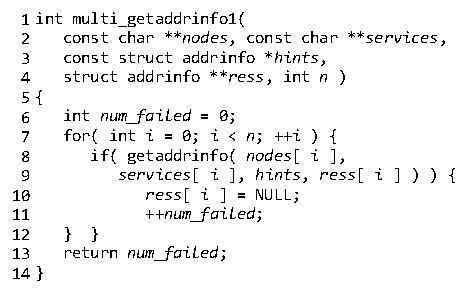
\includegraphics{multi_getaddrinfo_seq}
\caption{This is a plain C version of the DNS fetcher running example.
  This version is entirely \emph{sequential}.}
\label{fig:charcoal_multidns_seq}
\end{figure}

\begin{figure}
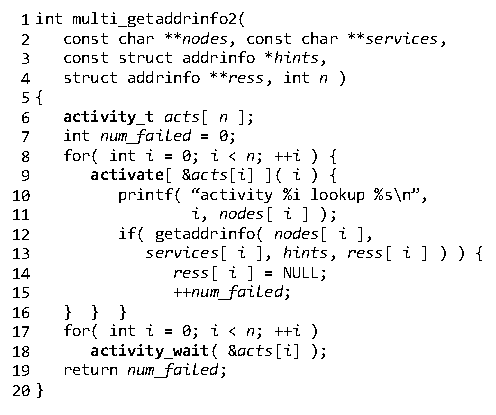
\includegraphics{multi_getaddrinfo_conc}
\caption{This is a \charcoal{} version of the DNS fetcher that sends all $N$ requests concurrently.}
\label{fig:charcoal_multidns_conc}
\end{figure}

To very briefly summarize \cite{Abadi2009}, the semantics of a program with activities can be seen as traces of actions separated by yield invocations.
Between two adjacent yield actions, all actions must come from a single particular activity.
Batches from different activities are interleaved by a scheduler to execute a complete program.
Actions are not permitted to cross yield boundaries.
In other words, yields define the minimum granularity of interleaving.

The system has a scheduler that chooses when a yield should lead to a context switch, and which activity to switch to.
The current \charcoal{} implementation uses a simple FIFO scheduler; clearly this is something that could be looked at for further refinement in terms of general performance, fairness guarantees and/or greater application control.

The activate statement takes as a parameter a pointer to application-allocated memory for storing metadata about the new activity.
In the example, the memory for storing activity information is allocated locally.
Because of this the example procedure must wait for all the activities it spawns to finish.
(Returning before they finish could cause the program to access deallocated memory).
It would be possible to change the interface so that the caller passes in the backing memory.
In that case, the procedure could return while the activities were still fetching DNS information, allowing the application to go on with other work.
In a language with automatic memory management, we would not have to be concerned about these memory allocation issues.

%% So far in this description, activities are identical to conventional cooperative threads.
%% \charcoal{} does have an explicit yield statement, though it is not often needed.

\subsection{Shared Variables}

Notice that multiple activities read and write the local variable \texttt{requested} without any additional synchronization.
If these were threads, this would cause a data race, which at best leads to unpredictable results and at worst make the whole program undefined.
With activities this is not a problem at all; the system (compiler, processors, etc.) is not permitted to move memory operations across yields, which dramatically simplifies the concurrent memory model problem.

The parentheses after the \texttt{activate} keyword are for controlling whether local variables are accessed by-value or by-reference.
The default is by-reference, which is how most of the variables are used in this example.
This means that all the activities read and write a shared instance of that variable.
The exception is \texttt{i} which is used as a name of sorts in the \texttt{printf} call.
Each activity gets its own copy of \texttt{i}, whose initial value is whatever the variable's value was at activity creation time.
If there were a modification to \texttt{i} inside \texttt{activate}, each activity would be modifying its own copy.

\subsection{Yield Insertion}

The primary feature that distinguishes activities from conventional cooperative threads is that there is a translation step that automatically inserts yield statements into the program before compilation or interpretation proper.
Figure \ref{fig:translation} shows some examples of the rules used to define where yields are inserted.
In general, yields are inserted on every back-edge in the control flow and before and after every call.
These rules guarantee that an activity cannot run indefinitely without invoking yield.

Implementing this correctly takes some care, because the compiler must be careful about things like \texttt{continue} and \texttt{goto} statements.

\begin{figure}
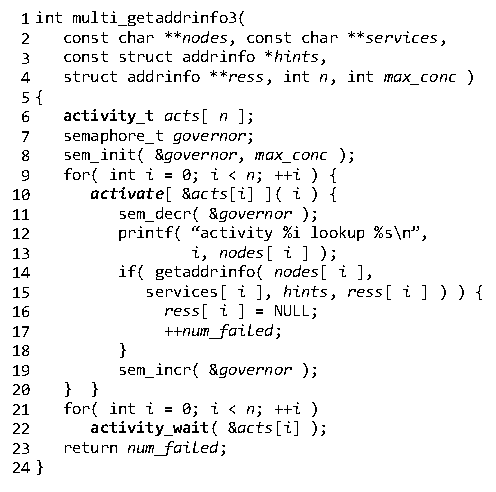
\includegraphics{multi_getaddrinfo_sem}
\caption{This version of the DNS fetcher limits the number of concurrent requests to \texttt{max\_conc}.}
\label{fig:charcoal_multidns_sem}
\end{figure}

In the example code above, the system will automatically insert five yields: one before the while loop jumps back to the beginning, and one each before and after the two calls.
The called functions themselves could have yields in their implementations.

Automatic yield insertion moves activities from cooperative threads towards preemptive threads from an application programmer's perspective.
However, activities are still more resistant to concurrency bugs than threads.
One reason for this is that the granularity of scheduling is coarser for activities.
Any block of code with acyclic control flow and no calls is guaranteed to execute atomically.

Though this minimum granularity may still seem quite fine, it does provide some nice properties.
Consider the classic data race example of two threads concurrently applying some arithmetic operation to a shared memory location.
Even if multithreading system were able to provide sequential consistency, it is possible for both threads to read the old value and end up with a result that would be impossible with coarser atomicity.
For this simple example there is no extra synchronization necessary with activities, which means that programmers can focus their attention on larger-scale issues.

\begin{figure}
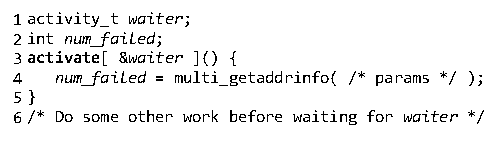
\includegraphics{multi_getaddrinfo_async_call}
\caption{This is a sketch of how an application can call a procedure asynchronously.
\texttt{waiter} and \texttt{num\_failed} would have to be heap-allocated if the application wanted to leave the current scope before the asynchronous call completes.}
\label{fig:charcoal_multidns_async_call}
\end{figure}

\begin{figure}
    \centering
    \begin{subfigure}[b]{0.5\textwidth}
  $e_f(e_1, \ldots, e_N) \Rightarrow$ \\
  \hspace*{1em} $( x_f=e_f; x_1=e_1; \ldots; x_N=e_N; \mathtt{yield};$ \\
  \hspace*{2em} $x_R=x_f(x_1, \ldots, x_N); \mathtt{yield}; x_R )$
        \caption{}
    \end{subfigure}
    ~ %add desired spacing between images, e. g. ~, \quad, \qquad, \hfill etc. 
      %(or a blank line to force the subfigure onto a new line)
    \begin{subfigure}[b]{0.5\textwidth}
  $\mathtt{while}( e ) \{ s \} \Rightarrow \mathtt{while}( e ) \{ s; \mathtt{yield} \}$
        \caption{}
    \end{subfigure}
    \caption{Examples of the translation rules used for yield insertion.
      (a) is the rule for function calls, and (b) is a part of the translation of while loops.}
    \label{fig:translation}
\end{figure}

There is one potential concurrency bug that this example avoids in a slightly subtle way.
The increment on line 11 must come before the call to \texttt{getaddrinfo}.
The system might context switch at that call, and it is important that other activities see the incremented version of the \texttt{requested} variable.
This example shows that activities are not immune to concurrency bugs, but avoiding them is easier than it would be in more flexibly scheduled abstractions.

%% These automatically-inserted yields make activities behave more like threads than events or coroutines from an application programmer's perspective.
%% However, there is a big difference between activities and threads.

%% %



%% Part of the definition of activities is that by default yields should happen ``frequently''.
%% But what does this mean precisely?
%% The answer depends on the details of the rest of the programming language definition.
%% However we can state two design rules that apply to any language.
%% These rules are in strong tension with each other:


%% One clear consequence of these rules is that anything that could cause an activity to pause indefinitely (e.g. a syscall) by default must be modified to allow other activities to run while the paused activity waits.
%% More challenging, loops must be interrupted.

\subsection{System Calls}

System calls present a challenge, because clearly a language cannot force the operating system to yield in the middle of kernel code execution.
To implement activities correctly, the system must ensure that system calls are performed asynchronously.
That is, during a system call the system may switch to another activity.
If a system call completes while some other activity is running, the calling activity must wait for a yield before it can resume execution.
There are more details on this in the implementation section.

\subsection{No-Yield}
\label{sec:noyield}

If there was no way to override yielding, activities would be little better than multithreading at resisting many kinds of concurrency defects.
To combat this \charcoal{} has no-yield.
Any statement, expression or procedure declaration can be ``wrapped'' with no-yield.
In the dynamic scope of a no-yield block, the current activity cannot be interrupted.
In other words, any yields that would have happened are overridden/suppressed by no-yield.
This is a simple and powerful tool for enforcing atomicity.
Most locking in current multithreading practice can be either removed entirely, thanks to the coarser scheduling granularity, or directly replaced by the simpler and safer no-yield.

In the example, the compiler will insert yields before and after the calls to \texttt{printf} and \texttt{getaddrinfo}.
If the programmer wanted to suppress some of these yields, they could use \noyield{}.
For example, it would be reasonable to wrap the \texttt{printf} call in \noyield{}, since it will complete quickly (relative to \texttt{getaddrinfo}), and there is little to be gained by switching to another task at that point.
Wrapping the \texttt{getaddrinfo} call in no-yield would be a performance bug, because that would force the DNS lookups to be executed sequentially.

\charcoal{} also has a variant of no-yield called no-implicit-yield.
This is a more subtle tool that is useful for high performance inner loop code.
The problem with such code is that yielding on every iteration causes non-trivial performance overhead, but yielding never (i.e. wrapping the whole loop in no-yield) could cause starvation.
Within the static scope of a no-implicit-yield block, yields are not automatically inserted, but explicit yields (those in the program source code) are not overridden.
There is an example of its use in the benchmarking section below.

%% \subsection{Recursive Procedure Calls}

%% The current design of \charcoal{} does not follow rule \#1 perfectly.
%% Function calls and returns do not implicitly yield, which means that recursion can be used to make an activity run indefinitely without yielding.
%% We consider this a bug, not a feature, in the language design, but we have not found any less bad alternatives.

%% The most obvious approach to avoiding yield-free recursion is to say that every call and/or return has an implicit yield.
%% This idea is bad for two reasons.
%% The simpler reason is that it violates rule \#2; calls and returns happen frequently in most programs and introducing a yield for every call would be very costly for performance.
%% The more important reason has to do with procedural abstraction.
%% If yields were inserted around calls, then the function extraction refactoring pattern would change the atomicity properties of the program.
%% This seems totally unacceptable.

%% One could imagine trying to identify recursive calls specifically and saying that only recursive calls carry an implicit yield.
%% However, with indirect calls it is impossible to precisely statically analyze which calls are recursive in general.
%% This means that the language design would have to codify some rules about which classes of calls could be guaranteed to be analyzed as recursive, which seems like a fragile design.
%% For C-like languages where recursion is used relatively sparsely in practice, this solution seems acceptable.
%% Programmers just have to be careful to insert yields in potentially long-running recursive procedures.
%% Functional languages would probably need to find a different compromise with regard to recursion.

\subsection{Activities, Compared}

In this section we describe important software engineering problems with existing multitasking abstractions and argue that activities avoid or substantially mitigate these problems.

\textbf{Events}.
Long-running callbacks (including those that might block indefinitely) must be \emph{manually} broken up into multiple callbacks.
This makes the logical flow of the program hard to reason about, both for programmers and analysis tools.
It can also make management of resources whose lifetime spans multiple callbacks quite tricky.
This leads to a style of programming referred to as \emph{stack ripping} \cite{Adya2002}, or more colloquially \emph{callback hell}.
These and more subtle problems are well analyzed and criticized by von Behren et al. in \cite{Behren2003a}.

One prominent ecosystem that uses callbacks heavily is Node.js.
In idiomatic Node.js code there are multiple nested higher-order function definitions that are passed around as callbacks.
This leads to code that is quite hard to read, but many in the Node.js community prefer this challenge to the problems associated with multithreading.

Like all variants of threads, activities allow tasks to be written in a more natural direct style, thus completely avoiding the problems associated with callbacks.
Events do maintain an advantage over activities in resistance to some concurrency defects, like atomicity violations.
However, the emergence of coroutines as an alternative to events is evidence that for many applications the costs described above have begun to outweigh the benefits.

\textbf{Coroutines}.
% Since widespread use of coroutines is much more recent than events and threads, there is far less published on their pitfalls.
From an implementation perspective, activities are actually quite similar to coroutines.
Procedure calls in \emph{no-yield mode} are like regular procedure calls in a coroutine framework.
In both cases, interruption is not allowed.
Procedure calls in \emph{yielding mode} are like coroutine ``calls''.

The main weakness of coroutines is most obvious during maintenance.
Assume that some function was originally written as a non-coroutine.
Later, things changed such that the function needed to perform some long-running actions and a programmer chooses to convert it from a regular procedure to a coroutine.
It is possible that this change will break atomicity assumptions made by the callers of this now-coroutine.

Stated slightly differently, with coroutines the atomicity of a call depends on the definition of the called thing.
With activities, the calling code can choose to wrap the call in no-yield or not, depending on its atomicity requirements.

A subtler difference has to do with defaults.
With coroutines, by default procedures are atomic, which means that accidental starvation/blocking is relatively easy.
With activities, by default any procedure call might be interrupted, which puts atomicity enforcement on the programmer to a greater extent.

Finally, coroutine frameworks have some awkwardness around the partitioning of procedures.
Regular procedures and coroutines are different things, so it is hard to use higher-order functional or object oriented patterns that abstract over whether something is a regular procedure or a coroutine.
With activities, all procedures are the same kind of thing and pointers to them can be passed around freely.

%% With the addition of no-yield, activities can be seen as quite similar to coroutines with a complementary default.
%% Normal procedures in an activity framework are like coroutines and normal procedures in a coroutine framework are like no-yield procedures in an activity framework.
%% As similar as this argument makes coroutines and activities seem, we believe the differences are still significant.
%% For example, in an activities framework, all procedures are part of the same type; normal procedures and no-yield procedures are not distinguished at the type level.

%% Coroutines have an interesting history.
%% According to Knuth, the term was coined by Melvin Conway in 1958, but coroutines remained on the margins of mainstream software practice until quite recently, a gap of more than 5 decades.
%% A few examples of recent implementations: the async/await framework (coroutines by a different name) was added to C\# in version 5, which was released in 2012; \texttt{function*} (coroutines by a different name) was added to the 2015 revision of ECMAScript; D4134 is a proposal to add coroutines to C++17.

%% Our interpretation of this history is that (1) coroutines are far from perfect as a multitasking primitive (otherwise they would have been widely adopted much sooner), and (2) mainstream applications have gotten more sophisticated in their use of multitasking, making life in callback hell ever more painful.
%% Coroutines are being adopted as the least bad alternative to events.

%% Using the coroutine abstraction requires application programmers to partition procedures into normal procedures (functions, methods, subroutines, whatever) and coroutines.
%% In most implementations the procedure calling syntax is overloaded; what appears to be a call to a coroutine is actually a concurrent task spawn.
%% Within the body of a coroutine definition, a \emph{yield} (or \emph{await}) primitive can be used to permit context switching to a different task (i.e. coroutine).
%% Invoking yield in a normal procedure is not permitted.

%% Relative to events, coroutines provide more flexibility, because multiple tasks can be in progress at the same time.
%% Coroutines are much more resistant to concurrency bugs than threads, because only one coroutine can be active at a time, and context switching is only permitted at explicitly identified points.

%% The primary weakness of coroutines is a subtle but nasty tension with conventional procedural abstraction.
%% It is common for application programmers to want to yield in a \emph{procedure} called by a coroutine, but this is not possible.
%% This can be quite inconvenient on its own, and it makes refactoring strategies like procedure extraction trickier to apply.
%% Another consequence of this issue is that coroutines tend to be viral; if a programmer decides to convert a procedure to a coroutine (for example because it needs to wait for the arrival of a network message), it tends to be the case that any callers of that procedure need to be converted to coroutines as well.

% Similarly, higher-order function patterns get more complicated as well.
% There are now two distinct types of procedure-like-things [clarify/expand].

% In languages with coroutines

%% These software engineering problems have not prevented the adoption of coroutines, but they do make it harder than it needs to be to develop multitasking software.
%% Activities solve these problems!

%% With the addition of no-yield, activities can be seen as quite similar to coroutines with a complementary default.
%% Normal procedures in an activity framework are like coroutines and normal procedures in a coroutine framework are like no-yield procedures in an activity framework.
%% As similar as this argument makes coroutines and activities seem, we believe the differences are still significant.
%% For example, in an activities framework, all procedures are part of the same type; normal procedures and no-yield procedures are not distinguished at the type level.

\textbf{Cooperative Threads}.
As explained above, activities are quite similar to conventional cooperative threads.
The primary weakness of cooperative threads is most prominent in large, complex applications.
The atomicity of a call depends on whether the called function (or any function it calls) invokes yield.
In small applications it is possible to investigate this manually and informally keep track of which functions might yield and which will not.
In large, evolving applications keeping track of these atomicity properties is extremely hard.
During maintenance this problem is especially prominent.
Adding (or removing) a yield can have large effects on the potential for concurrency defects, and the programmer needs to understand all of the contexts in which a particular procedure might be called.

With activities, programmers must assume that any call might yield, unless the called function is explicitly marked no-yield.
This makes the decision process simple: if interruption during a particular call is unacceptable, the programmer must wrap it in no-yield.

%% Cooperative threads are not as widely used as events, threads and coroutines, but we briefly describe them because they are closely related to activities.
%% Cooperative threads can be seen as a compromise between coroutines and threads.
%% Like coroutines, cooperative threads must explicitly invoke a yield primitive to context switch.
%% Like threads, cooperative threads do not have a separate kind of procedure (i.e. coroutine/async) and yield can be invoked anywhere (i.e. it is not restricted to coroutine bodies).

%% Cooperative threads have a tension with procedural abstraction that is complementary to the tension in coroutine abstractions.
%% Whether a particular procedure executes atomically depends on whether or not any of the procedures it calls will invoke yield.
%% This can be annoying when initially writing code, and it is especially problematic during maintenance.
%% If yield is added to a procedure that did not previously have it, there is the possibility that any caller of that procedure will have its atomicity properties violated.
%% This is extra nasty when indirect calls are considered, because it is not possible in general to identify all call sites to a particular procedure.

\textbf{User-level Threads (Preemptive)}.
Activities are similar in many ways to user-level threads.
Some user-level thread implementations provide a \emph{disable-interrupts} primitive that is quite similar to our no-yield.
The critical difference between threads and activities is when interruptions can happen.
Conventionally, user-level threads can be interrupted at any point during execution.
Among other problems, this can lead to data races, which can lead to a wide range of surprising problems (see for example \cite{Boehm2011}).
Like every abstraction in the cooperative thread family, activities cannot suffer from data races; it is a complete non-issue.

Using special compilation strategies it is possible to systematically eliminate most defects associated with data races.
For example, see \cite{Singh2012} where a ``sequential consistency preserving'' compiler that avoids or limits many optimizations in the name of concurrency bug resistance is described.
We are not aware of any implementations of this idea outside of a few research projects.
As described above, the coarser scheduling of activities provides greater resistance to fine-grained atomicity violations than sequential consistency.

The idea of automatic insertion of yields to make cooperative threads more like preemptive threads has been investigated before.
For example, Boudol proposes such a language in \cite{Boudol2007}.
His focus was on using analysis techniques to reduce the frequency of inserted yields, without giving up the guarantee that a thread cannot run indefinitely.
Rather than relying on a sophisticated compiler to make these choices, we prefer to put the power in the hands of the programmer with \emph{no-yield}.
It is possible for programmers to create starvation problems with poor uses of no-yield, profilers can easily track the duration of no-yield blocks and warn about those that take too long.

\textbf{Threads (System)}.
The most obvious difference between activities and threads is that activities cannot easily be run in parallel.
This is clearly not a fatal flaw for multitasking abstractions, since event handlers and coroutines also cannot be run in parallel.
See the related work section for further discussion of parallelism and its relationship to multitasking.

System threads are almost identical to preemptive user-level threads from a software engineering perspective, except they are somewhat more diabolical.
Because system threads can be run in parallel, actions from different threads tend to be interleaved in a much more fine-grained way than they would be with non-parallel threads.
This does not categorically change what kinds of defects are possible, but it does make things like data races and atomicity violations more likely to occur in a particular execution.

\textbf{Threads Plus Transactions}.
Comparing activities to any flavor of preemptive multithreading, the impossibility of data races eliminates some of the need for synchronization immediately.
However, other kinds of defects like atomicity violations are still a potential problem.
The no-yield primitive provides a much better way of avoiding these defects than conventional locks.
No-yield is quite similar to atomic blocks in transactional concurrency control languages.
Atomic blocks have been shown to make avoiding concurrency defects easier (see, for example \cite{Harris2005, Grossman2007}.
\emph{No-yield} has a couple of advantages over \emph{atomic}.
First, there are no thorny semantic issues with memory that is accessed both inside and outside of no-yield mode.
Second, no-yield blocks are never executed speculatively, which means that there are no problems with performing I/O operations in no-yield mode.

%% Events are at the safest and least flexible end of the multitasking abstraction spectrum and threads occupy the opposite extreme.
%% (In this paper \emph{thread} means \emph{preemptive thread}.)

%% The primary strength of threads is that they can wait/block indefinitely or run for an arbitrarily long time without preventing other threads from making progress.
%% This makes it possible to write multitasking software in a natural single-task style (i.e. threads completely avoid callback hell).

%% The primary weakness of threads is that it is extremely hard to avoid and debug concurrency defects like data races, deadlocks, atomicity violations and livelocks.
%% In the last decade a significant amount of research effort has been devoted to making it easier to write reliable multithreaded applications, because of the emergence of mainstream multiprocessor computers.
%% While this body of work is quite impressive, most mainstream application programmers still view threads as too dangerous for multitasking programming (correctly in the current authors' opinion).

%% Applications that use threads and conventional concurrency control mechanisms also suffer from serious composability issues \cite{Harris2005, Grossman2007}.
%% The very brief summary of the arguments in the cited papers is that when using mutexes, semaphores and their cousins, application programmers must design and (somehow) enforce subtle global concurrency control properties.
%% Using transactions instead of conventional concurrency control mechanisms promises to make threads safer and more composable.
%% Unfortunately, questions about how transactions should interact with input/output and performance/scalability concerns have severely limited the adoption of general purpose transactional concurrency control.

\section{Implementation}

There are a few interesting features of our implementation of activities.
The the following sections we describe the allocation of call frames, the implementation the yield primitive, and compiling a version of each procedure for yielding and no-yield mode.

\subsection{Call Frame Allocation}

One of the tricky issues in the implementation of any thread-like abstraction is the allocation of procedure call frames.
The first few sections below describe existing strategies for frame allocation in multithreaded code.
Then we describe a new approach that we call \emph{hot stacking}.

\subsubsection{Contiguous Allocation}

In single-thread applications it is convenient and efficient to allocate \emph{the} stack of call frames contiguously in a single large region of memory.
% This works well because the live ranges of frames are strictly nested; a callee's frame is deallocated before its caller's.
This strategy cannot be directly used for multithreaded applications, because each thread needs to allocate and deallocate frames independently.

The most common strategy for multithreading is to pre-allocate a moderately large area of memory in the heap for each thread's frames.
Individual frames are allocated contiguously within this area.
This strategy is fast and simple, but it has a nasty tension with memory efficiency.

If the allocated areas are too small, the application will experience stack overflows.
If the allocated areas are too large, a significant amount of (virtual) memory is wasted.
In practice most existing multithreaded software takes a conservative approach, allocating much larger areas for stacks than is strictly necessary.

Especially in 64-bit address spaces, the wasted virtual memory space is not an acute problem.
However, because memory is typically allocated in page-sized chunks this allocation strategy wastes the physical memory between the top of the stack and the end of the page that it happens to be in.
This can easily mean a couple of wasted kilobytes per thread.

These memory efficiency issues are one reason that most mainstream applications use only a few threads, and very few applications use more than a few dozen.
For software architectures that might require more than this limit, thread pooling is a common solution.
However, thread pooling brings its own inefficiencies and software engineering challenges.

\subsubsection{Individual Heap Allocation}

A completely different approach to frame allocation is individually allocating each frame in the heap.
This avoids the memory concerns associated with contiguous allocation.
However, heap allocation of frames comes at a significant performance cost for call and return operations.

Simple implementations of heap allocation are generally more than an order of magnitude slower than contiguous allocation (see more details in the microbenchmarking section below).
More sophisticated implementations can be substantially more efficient (e.g. \cite{Shao2000}).
However, even the most efficient implementations that we are aware of are still substantially slower than contiguous allocation for call-heavy code.

\subsubsection{Split/Segmented Stacks}

Some languages have experimented with a hybrid strategy called \emph{split}, \emph{segmented}, or \emph{linked} stacks.
The idea is that stack space is allocated in small segments.
The common case call/return execution looks like traditional contiguous allocation.
When a thread reaches the end of its segment it allocates a new one and links them together.
This idea is appealing: the implementers of Rust and Go both used it.
Unfortunately it has really unpleasant \emph{uncommon} case behavior called \emph{stack thrashing} or \emph{the hot split problem}.
When there are frequent calls/returns right at the boundary of a segment, the overhead can be quite high.
The implementers of Rust \cite{Anderson2013} and Go (search ``contiguous stacks in go'') both abandoned split stacks in later versions.

% Also \cite{Middha2008}

\subsubsection{Dynamic Contiguous Stacks}

Since version 1.3, the Go language has used a novel stack allocation strategy, where each thread's stack memory is initially small and is resized on-demand.
This is only possible because the Go language implementation knows about all pointers to stack memory and can update them if necessary (i.e., if it is necessary to relocate the whole stack).
Clearly this would not work for C/C++ and close cousins.
Even this strategy has non-zero overhead for call/return, as we show in the benchmark section below.

\subsubsection{Hot Stacking}

The call frame allocation strategy introduced in this paper is a hybrid of contiguous and individual heap allocation.
The primary observation is that the slowness of individual allocation is only important for short-lived calls.
For long-lived calls (generally calls nearer the base of the call stack), the overhead of the call and return operations can be amortized over the long running time of the call and its callees.
So the main idea of hot stacking is that long-lived frames are individually allocated and (most) short-lived frames are contiguously allocated in memory that is shared by multiple activities.

For this strategy to work correctly, the frames allocated in the shared area must all be deallocated before context switching to another task.
For regular threads it is not clear how this deallocation could be enforced easily.
Activities make it practical to use hot stacking, because the implementation can use no-yield blocks as an indicator of when it should use contiguous allocation.
Context switches are not permitted in no-yield mode, so there is no problem with needing to context switch when frames in the shared area are still in use.

In the microbenchmarking section below we provide evidence that this strategy captures the benefits of heap allocation (per-activity memory overhead is very small) and contiguous allocation (fast calls and returns when it matters most).
It is certainly possible for short-lived calls to happen in yielding mode, which means that the frames will be individually allocated.
This should be considered a performance bug, but its worst-case overhead is not terrible and it should be a relatively easy pattern to identify with a profiler.

The name \emph{hot stacking} is a reference to a practice used in some military and business organizations called \emph{hot racking} or \emph{hot desking}.
Some limited resource (e.g. a bunk or desk) is used in shifts by multiple people.
In our case, the resource is the memory area for contiguous frame allocation, and it is shared in shifts by multiple activities.
The word \emph{hot} is also a reference to the fact that this top of stack area should remain hot in the memory hierarchy/cache sense as long as any code is running.

\subsection{Yield Implementation}
\label{sec:yield_imp}

Since automatic yield insertion makes it so that by default yields happen quite frequently, we need to ensure that yields are as efficient as possible.
In particular, we implemented three ideas:

\begin{itemize}
\item Zero overhead yields in no-yield mode
\item Infrequent context switching
\item Very fast non-switching yield
\end{itemize}

\subsubsection{Yield in No-Yield Mode}

There are important differences at the implementation level between how code executes in yielding versus no-yield mode, not least among them the call frame allocation strategy.
To implement this dual mode concept in a reasonably simple and efficient way, the current \charcoal{} implementation generates two versions of each procedure: one for each mode.
The yielding mode implementation includes inserted yields and assumes its own frame was individually allocated.
The no-yield mode implementation does not include yields; for most intents and purposes it is a simple translation to plain C.

Of course making a single implementation that could be run in either mode would be possible.
Such an implementation would need to branch on which mode it was running, potentially quite frequently.
This seemed like a performance killer for inner loop code, though we have not investigated this assumption yet.

This implementation strategy could lead to a substantial increase in code size.
We have two ideas about how this can be avoided, though we have not investigated either yet.
First, most procedures are only called in either one mode or the other.
A sufficiently smart linker could identify the version that is never called and eliminate it.
Second, in language implementations that already do runtime optimization, the (static) compiler could only generate yielding mode versions and leave it up to the runtime code generator to make no-yield versions for procedures that are actually called in no-yield mode.

%% This is kinda related to ideas from the Cilk-5 implementation
%% \cite{Frigo1998}.

\subsubsection{Function Pointers}

One challenge with a dual implementation strategy is how to handle function pointers.
In general, when the address of a function is taken there is no way to know which mode the function will later be called in.
Therefore simply taking the address of either implementation would be at best complicated and inefficient, and quite likely lead to subtle bugs.
The current implementation generates a small piece of code for every function that can be called in either yielding or no-yield mode.
A parameter is passed by the caller to indicate which mode it is in.
The generated code calls the appropriate implementation.
This makes indirect calls somewhat more expensive than in plain C.
However, indirect calls are already expensive enough that there is an extensive body of research on how to convert them to direct calls (e.g. \cite{Dean1995}), so adding a modest amount of overhead to indirect calls should not have a large performance impact on most applications.

\subsubsection{Yields}

The most important factor in the implementation of the yield primitive is that most yield invocations should not result in context switching, even if other activities are ready to run.
In well designed activity code, the time between yield invocations should be in the range of microseconds to milliseconds.
Context switching has the moderate direct cost of manipulating a handful of data structures in the runtime system, and the potentially higher indirect cost of cache thrashing.
Therefore in normal operation yields should lead to context switches at a relatively low frequency, perhaps every few milliseconds.

The speed of the yield primitive itself is somewhat important.
As described in the previous section, code that is compiled in no-yield mode does not have yields at all, so yield performance is not an issue for the most performance critical loops.
However, we expect that moderately frequent yielding (perhaps as frequently as many per microsecond) would be common in real-world code.
Therefore, the performance of the yield primitive does matter to some degree.

The simplest implementation of yield would check a counter or clock of some sort.
Reasonably efficient implementations of this strategy would certainly be non-portable (e.g. using processor-specific counter registers) and probably still be somewhat expensive.
Instead the current \charcoal{} implementation uses periodic system timers/alarms that deliver a signal to the program.
The handler for these signals atomically modifies a global variable.
The yield primitive atomically reads this global variable; as long as it has not changed the program continues execution immediately.
Therefore, in the common case the cost of a yield is only an atomic read and a (highly predictable) branch, plus a fast call and return to get to the yield code itself.
(Of course the yield code can be inlined, but that is \emph{not} obviously a good idea because the branch prediction hardware works much better if all yields share a single branch instruction.)

\subsection{Asynchronous System Calls}

An important part of making activities work properly is asynchronous system calls.
The current \charcoal{} implementation uses libuv for this.
At startup, the runtime system spawns a thread that runs a libuv event loop.
When an activity wants to make a system call, it sends an asynchronous message to the event loop thread, which makes the appropriate libuv API call.
When the event completes, the activity is notified and the system puts it back in the runnable queue.

This architecture works, but it adds a non-trivial amount of overhead, especially for reasonably fast system calls.
We speculate that integrating the event processing with application code in the same thread could remove some performance overhead.
The libuv maintainers have discussed this as a ``pull'', versus the current ``push'' architecture, which they may implement in a future version.

\subsection{Translation}

We use a modified version of Cil \cite{Necula2002} to translate \charcoal{} to plain C with calls to our runtime system.

\section{Benchmarking}

To establish the practicality of activities, we implemented 5 microbenchmarks.
All tests were run on a machine with the specs listed in Table \ref{table:specs}.
Depending on the benchmark, we compare the \charcoal{} implementation against plain C, C compiled with gcc's split stack implementation, Go or C plus the default Linux threads implementation.
All speed-related tests were compiled at optimization level \texttt{-O2}.
For speed-related tests we ran the benchmark 5 times and report the fastest result.

\begin{table}
  \centering
  \begin{tabular}{|l|l|}
    \hline
    OS & Ubuntu Linux 14.04 \\
    \hline
    Kernel & 3.13.0-68-generic \\
    \hline
    Processor & 4 GHz Intel Core i7 \\
    \hline
    Memory & 8 GB 1600 MHz DDR3 \\
    \hline
    Compiler & gcc 4.8.4 \\
    \hline
    Go & 1.5.3 \\
    \hline
  \end{tabular}
  \caption{Specs of the test system}
  \label{table:specs}
\end{table}

\subsection{Task Memory Overhead}

The first microbenchmark measures memory overhead by spawning tasks until memory is exhausted.
For activities this overhead is small and more or less fixed.
For threads this overhead is harder to put a single number on, because most multithreading APIs allow the amount of memory reserved for the call stack to be controlled by the application.
For this benchmark we used the default stack size.

\vspace{1em}
\begin{tabular}{|l|r|}
  \hline
  Threads & 31,000 \\
  \hline
  Goroutines & 9,200,000 \\
  \hline
  Activities & 61,000,000 \\
  \hline
\end{tabular}
\vspace{1em}

By this measure, the memory overhead of activities is more than 3 orders of magnitude smaller than threads.
The results of this test are not surprising, but we believe it is worth emphasizing that in most contexts it is not practical to use more than a few hundred or maybe a few thousand threads.

A closer comparison is between activities and goroutines.
The Go implementation (as of version 1.3) uses a sophisticated stack growing process to avoid pre-allocating large regions of memory for call frames.
However, the minimum size is still relatively large (in the neighborhood of a kilobyte), more than a factor of 6 greater than activities in \charcoal{}.
We would expect to find a similar minimum overhead in implementations that use split/segmented/linked stacks.

%% Some would argue that having so many thread-like things active simultaneously is not good software architecture anyway.
%% We do not argue that point here, but just point out that lower memory overhead can only be better.

\subsection{Task Spawn Speed}

% wait for previous task
% spawn new task

The second microbenchmark measures how quickly new tasks can be spawned.
In this test each task waits for the previous task to finish, then spawns the next task.

\vspace{1em}
\begin{tabular}{|l|r|r|r|}
  \hline
   & user & sys & wall \\
  \hline
  \hline
  Threads & 3.2 & 45.9 & 35.6 \\
  \hline
  Goroutines & 0.39 & 0.003 & 0.40 \\
  \hline
  Activities & 0.31 & 0.002 & 0.31 \\
  \hline
\end{tabular}
\vspace{1em}

All numbers are given in microseconds per spawn.
The difference between threads and activities in this test is over two orders of magnitude.
Also interesting to note is that the majority of the time for threads is used in the operating system, whereas the system time for activities is negligible.
The thread implementation gets a small benefit from processor parallelism, whereas the activity implementation does not (of course).

Spawn overhead is important because it determines the minimum granularity of work for which a task can (efficiently) be spawned.
With a spawn time well under a microsecond, programmers would only have to worry about this overhead in extreme cases where an activity only executed a few instructions before finishing.
% In other words, there is little reason to manage \emph{activity pools}; it is almost always a better idea to simply spawn a new activity for the task at hand.

\charcoal{} is barely faster than Go in this benchmark.
We do not consider this difference to be large enough to be interesting.
% We believe this is primarily due to a more optimized implementation, not differences between the abstractions.
% We expect that this gap could be closed with more work on the \charcoal{} implementation.

\subsection{Task Switching}

The third microbenchmark measures how quickly the system can switch from one task to another.
For this test we spawned 100 tasks and organized them in a ring, each waiting for a signal of some kind from its neighbor.
The test injects a signal at one point and then measures how quickly it can cycle around the ring.

\vspace{1em}
\begin{tabular}{|l|r|r|r|}
  \hline
   & user & sys & wall \\
  \hline
  \hline
  Threads & 0.00 & 7.8 & 12.1 \\
  \hline
  Goroutines & 0.19 & 0.00 & 0.20 \\
  \hline
  Activities & 0.22 & 0.00 & 0.23 \\
  \hline
\end{tabular}
\vspace{1em}

These numbers are in microseconds per task switch.
The pattern here is similar to the previous test.
Activities are well over an order of magnitude faster than threads.
% We do not know why for threads the wall clock time reported by the time utility is higher than the sum of the user and system times.
Like the spawning benchmark, the main conclusion is that the overhead for activities is low enough that individual activities can do quite small units of work per context switch without paying a high overall efficiency penalty.
% This opens the door to software architectures with many activities organized in a dataflow computing style.

Again, Go has a small performance edge on \charcoal{}, which we attribute to maturity of the implementation.

\subsection{Just Calling}

The fourth microbenchmark measures the overhead of the hot stacking allocation strategy.
This test is a simple recursive function that calls itself twice and performs a very small computation at the ``leaves''; the code is in Figure \ref{fig:micro_calling}.

\vspace{1em}
\begin{tabular}{|l|r|r|r|}
  \hline
   & user & sys & wall \\
  \hline
  \hline
  Plain C & 0.77 & 0.00 & 0.77 \\
  \hline
  Individual Allocation & 42.4 & 0.04 & 42.6 \\
  \hline
\end{tabular}
\vspace{1em}

These numbers are in nanoseconds per call/return.
This difference is nearly two orders of magnitude, which is painful for \charcoal{}.
However, there are several caveats to keep in mind.
First, the \charcoal{} implementation is not highly optimized; in particular the allocator used in this test was just the default system malloc.
Surely a more tuned implementation would close the gap to some extent.
Second, this is a microbenchmark; no application spends all of its time just calling and returning, so these numbers are a fairly high upper bound on the real application performance impact of calling overhead.

\begin{figure}
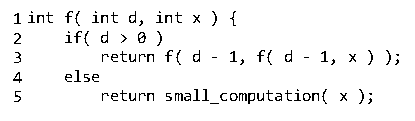
\includegraphics{just_calling_benchmark}
\caption{The microbenchmark for measuring call frame allocation overhead.}
\label{fig:micro_calling}
\end{figure}

Most importantly, all the calls in the first version of this test were performed in yielding mode.
In no-yield mode, calls and returns in \charcoal{} are just as efficient as plain C.
In well-tuned \charcoal{} code, most of the leaf and near-leaf calls should be performed in no-yield mode.
To simulate this effect, we modified the benchmark to the version in Figure \ref{fig:micro_calling_n}.
The parameter \texttt{N} controls how deep in the call tree the benchmark uses yielding mode, before switching to no-yield.

\vspace{1em}
\begin{tabular}{|l|r|r|r|}
  \hline
   & user & sys & wall \\
  \hline
  \hline
  Plain C & 0.77 & 0.00 & 0.77 \\
  \hline
  gcc split stacks\footnotemark{} & 1.00 & 0.15 & 1.15 \\
  \hline
  Go & 2.80 & 0.20 & 3.00 \\
  \hline
  Hot Stacking, \texttt{N} = 4 & 11.00 & 0.01 & 11.00 \\
  \hline
  Hot Stacking, \texttt{N} = 8 & 1.54 & 0.00 & 1.55 \\
  \hline
\end{tabular}
\vspace{1em}

\footnotetext{This benchmark does not create stacks deep enough to exceed the default size of a single segment of gcc's split stack.
So we modified the benchmark for the split stack case to make a linear chain of calls instead of a binary tree.}

This shows that with a modest fraction of the (static) calls performed in no-yield mode, the calling overhead gets down to less than a factor of 2.
Combined with the observations above about tuning the language implementation and real application performance, we believe this overhead is tolerable for most applications.
Also it is worth noting that this is the price to be paid for the extremely low memory overhead of activities.

Hot stacking with \texttt{N} = 8 outperforms Go on this benchmark by a modest margin.
It is interesting that the gap between plain C and Go is as large as it is, given the Go implementation team's famous focus on low-level performance details.

gcc's split stack implementation outperforms hot stacking by a small margin on this benchmark.
However, split stacks have bad performance in the pathological case where calls are made at high frequency right at the edge of a segment.
The Rust community calls this ``stack thrashing''; the Go community calls it the ``hot split'' problem.
Hot stacking does not suffer from this problem.

\begin{figure}
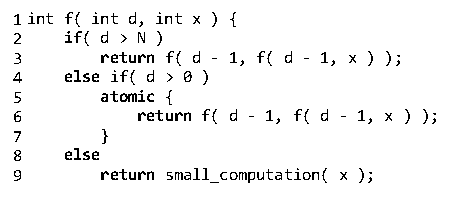
\includegraphics{just_calling_n_benchmark}
\caption{The call/return microbenchmark modified to make some calls in no-yield mode.}
\label{fig:micro_calling_n}
\end{figure}

\subsection{Yielding}

As described in section \ref{sec:yield_imp}, yielding is made fast by two tricks:
First, when the compiler generates no-yield mode code, it simply does not insert yields at all.
Second, the fast common case for yielding is just performing an atomic read on a global variable and branching.
Even with this fast implementation, yielding is still not free.
It is important to avoid yielding in hot inner loops.

To quantify this overhead, we benchmarked a simple but problematic function from the C standard library: \texttt{strcmp}.
\texttt{strcmp} is tricky for a few reasons:
First, the input strings can be arbitrarily long, so never yielding is not acceptable.
Second, the body of the loop is extremely simple; good implementations are just a few assembly instructions.
This means that yielding every iteration causes significant performance overhead.
Third, the continued execution of the loop depends on the data read in each iteration, so simple loop tiling/blocking tricks do not work.
The best-performing implementation we have found so far appears in Figure \ref{fig:strcmp}.

\begin{figure}
    \centering
    \begin{subfigure}[b]{0.3\textwidth}
        \hspace{-1.5cm}
        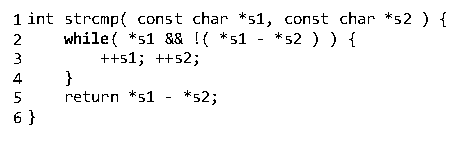
\includegraphics{plain_strcmp}
        \caption{}
    \end{subfigure}
    ~ %add desired spacing between images, e. g. ~, \quad, \qquad, \hfill etc. 
      %(or a blank line to force the subfigure onto a new line)
    \begin{subfigure}[b]{0.3\textwidth}
        \hspace{-1.5cm}
        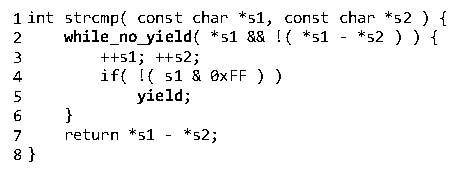
\includegraphics{strcmp_benchmark}
        \caption{}
    \end{subfigure}
    \caption{Two implementations of \texttt{strcmp}.
      (a) is a plain C version.
      (b) is a \charcoal{} implementation aimed at minimizing yield overhead. }
    \label{fig:strcmp}
\end{figure}

\texttt{no\_implicit\_yield} is a special variant of no-yield, described in section \ref{sec:noyield}.
In this case the compiler will not insert yields at the end of the while loop iterations.

In the code \texttt{YIELD\_FREQ} controls how frequently the loop yields.
The effect is that once every $2^{\mathtt{YF}}$ iterations there is a yield.

\vspace{1em}
\begin{tabular}{|l|r|}
  \hline
  Plain C & 430 \\
  \hline
  \charcoal, \texttt{YIELD\_FREQ = 4} & 1070 \\
  \hline
  \charcoal, \texttt{YIELD\_FREQ = 8} & 519 \\
  \hline
  \charcoal, \texttt{YIELD\_FREQ = 12} & 446 \\
  \hline
\end{tabular}
\vspace{1em}

These numbers are in microseconds per \texttt{strcmp} of two identical strings of 1MB length.
These data show that yielding is far from free, but with a little careful tuning the yield overhead can be brought quite low.
Recall that yield frequency can be as low as about once per millisecond without negatively affecting the responsiveness of most applications, so yielding every 4k iterations (as in the \texttt{YIELD\_FREQ = 12} case) is fine.

When the inputs to \texttt{strcmp} are known to be short, the caller can wrap the call in no-yield.
The no-yield version should perform identically to the plain C implementation.

% \subsection{Code Size}

\subsection{Microbenchmark Summary}

Like all well implemented coroutines/cooperative threads, the \charcoal{} implementation has extremely low memory and time overhead for basic concurrency primitives.
Hot stacking and frequent yielding are potential performance issues, but our tests indicate that at these overheads can be managed.

Though we do not have experience with writing large programs in \charcoal{} yet, we expect that relatively little code will require the kinds of contortions shown in the \texttt{strcmp} example.
Moreover, almost all such code will be in tight inner loops in library code.
This is exactly where writing somewhat weird code for performance reasons is acceptable.

%% \section{Foreign Code}

%% Foreign code (including legacy code) will never yield.  This could lead
%% to starvation pretty easily.  Here are three strategies:

%% \begin{itemize}
%% \item Do nothing.
%%   Just run the foreign code.
%%   This is a perfectly reasonable strategy as long as the foreign code does not run for a long time.
%% \item Run the foreign code in its own thread.
%%   If it has not returned by the end of some time slice, pause it to allow other activities to run.
%%   This runs the risk of creating atomicity violations galore.
%%   It also reintroduces the possibility of data races.
%%   However, it might be a reasonable strategy in situations where there is very little sharing between the foreign code and the rest of the application.
%% \item Run the foreign code in its own thread, but only interrupt it at special ``safe-ish'' points, like system calls.
%%   This is a compromise between the previous two strategies in the sense that it opens the door to both starvation and atomicity violations, but provides some (imperfect) protection against both.
%% \end{itemize}

%% We have not thought at all about what the best default is or what syntactic sugar would be nice.

%% Another important implementation issue to consider is foreign code that calls back in to activity-aware code.
%% There will definitely be some fancy footwork necessary there, no matter which strategy is used.

\section{Related Work}

As mentioned in the introduction, there are many projects that have aimed for a hybrid somewhere between threads and events.
One of the closest to the system reported here is Continuation Passing C (CPC) \cite{Kerneis2013}.
In that work the authors focus on the ability to switch back and forth between preemptive and cooperative modes, rather than a single abstraction that combines the best of both.
In some of the CPC publications, the designers claimed that it was not possible to implement some more exotic features of C, like setjmp/longjmp and alloca.
A detailed description of our implementation of these features is beyond the scope of this paper, but a working implementation is available in the project repository.
The hot stacking frame allocation strategy makes the implementation of these features (and related things like exceptions) more complicated, but not impossible.

One weakness that activities share with most multitasking frameworks is that activities cannot easily be run in parallel.
Naively running activities simultaneously on parallel processors would immediately violate the simple sequential memory model.
However, it is interesting to consider what it would take to run activities in parallel without violating their semantics.
The most obvious way to accomplish that would be with a transactional memory system; every activity would always be running in a transaction.
Yielding would cause one transaction to end and the next to begin.
The authors are not optimistic that such a transaction based system would work well, but other researchers are pursuing this kind of idea \cite{ONeill2015, Boussinot2006, Dabrowski2006}.

Our opinion is that parallelism should be accomplished with isolated processes.
Units of work can be dispatched to multitasking primitives (like events, coroutines or activities) running in isolated worker processes.
This is not a simple software architecture, but it does provide processor parallelism while largely avoiding the nasty mess of shared memory parallelism.

%% Threads are the only multitasking abstractions discussed in this paper that naturally allow the parallel execution of tasks.
%% The authors view this as closer to a bug than a feature.
%% Serial multitasking abstractions like events and coroutines (and activities) can be used in combination with parallelism frameworks like processes and threads.
%% The authors consider providing both parallelism and multitasking in a single language features (like threads) mostly a bad idea.
%% Nevertheless, in the discussion section at the end of this paper we speculate about the feasibility of running activities in parallel.


% Threads without the Pain

\subsection{Other Multitasking Abstractions}

There are multitasking abstractions that we did not analyze earlier in the paper.
We mention them briefly here, only to argue that they are more distantly related for one reason or another.

\textbf{Isolated processes}.
Isolated process can be used for multitasking.
However, for things like handling GUI events, database transactions and network communication, shared memory is an extremely useful feature.

\textbf{Functional reactive programming}.
Functional reactive programming (FRP) is an entirely different approach to multitasking.
The central idea is that observable outputs are pure functions (potentially very complicated ones) of live inputs.
This is an interesting idea, but it is not clear whether it can be implemented efficiently and integrated with mainstream programming practice.

\textbf{Dataflow langauges}.
Languages like Lustre, Esterel and Ptolemy provide a completely different approach to programming.
These kinds of languages are used somewhat in embedded systems, but are barely used at all in mainstream application programming.

\section{Summary and Discussion}

In this paper we introduced pseudo-preemptive threads/activities, a new multitasking primitive.
Activities have advantages in reliability, composability and/or maintainability over the most common approaches to writing multitasking software (events, threads and coroutines).
From an application programmer's perspective activities feel most like threads, but they do not suffer from several of the nasty concurrency problems that plague multithreaded software.
Activities also have extremely low memory and time overheads compared to conventional thread implementations.
Activities can be thought of as actually working the way inexperienced programmers think threads should work, which we think is a good thing.

% \acks

% Acknowledgments, if needed.

% We recommend abbrvnat bibliography style.

% \bibliographystyle{abbrvnat}
\bibliographystyle{abbrv}

% The bibliography should be embedded for final submission.

\bibliography{../../../../Documents/PapersForReferencing/biy_all_research.bib}

%% \begin{thebibliography}{../../../../Documents/PapersForReferencing/biy_all_research.bib}
%% \softraggedright

%% \end{thebibliography}

\end{document}
